\documentclass[a4paper, 12pt]{article}

\usepackage[top=2cm, bottom=2cm, left=2.5cm, right=2.5cm]{geometry}
\usepackage[utf8]{inputenc}
\usepackage{array}
\usepackage{cancel}
\usepackage{graphicx}
\usepackage{amsmath}

\graphicspath{{img/}}

\begin{document}
\begin{flushleft}
\includegraphics{logo}\\
\textbf{UNIVERSIDADE ESTADUAL DE PONTA GROSSA} \\
SISTEMA UNIVERSIDADE ABERTA DO BRASIL - UAB \\
\underline{Licenciatura em Matemática | Polo UAB em Jacarezinho}\end{flushleft} 
\textbf{ALUNO:} Ricardo Medeiros da Costa Junior   \textbf{RA:} 151774301 \\
\textbf{DISCIPLINA:} Fundamentos da Matemática III \\
\textbf{ATIVIDADE:} Atividade 8 - Tarefa: Equações Polinomiais\\
\textbf{TUTOR(A)}: Julio Cezar de Souza\\
\textbf{PERÍODO:} Terceiro\\
\begin{enumerate}
\item Elabore cinco questões envolvendo a obtenção das raízes de equações polinomiais.\\
  \begin{enumerate}
  \end{enumerate}
\item Em seguida apresente graficamente as soluções reais. \\
    \begin{figure}[h!]
    \centering
    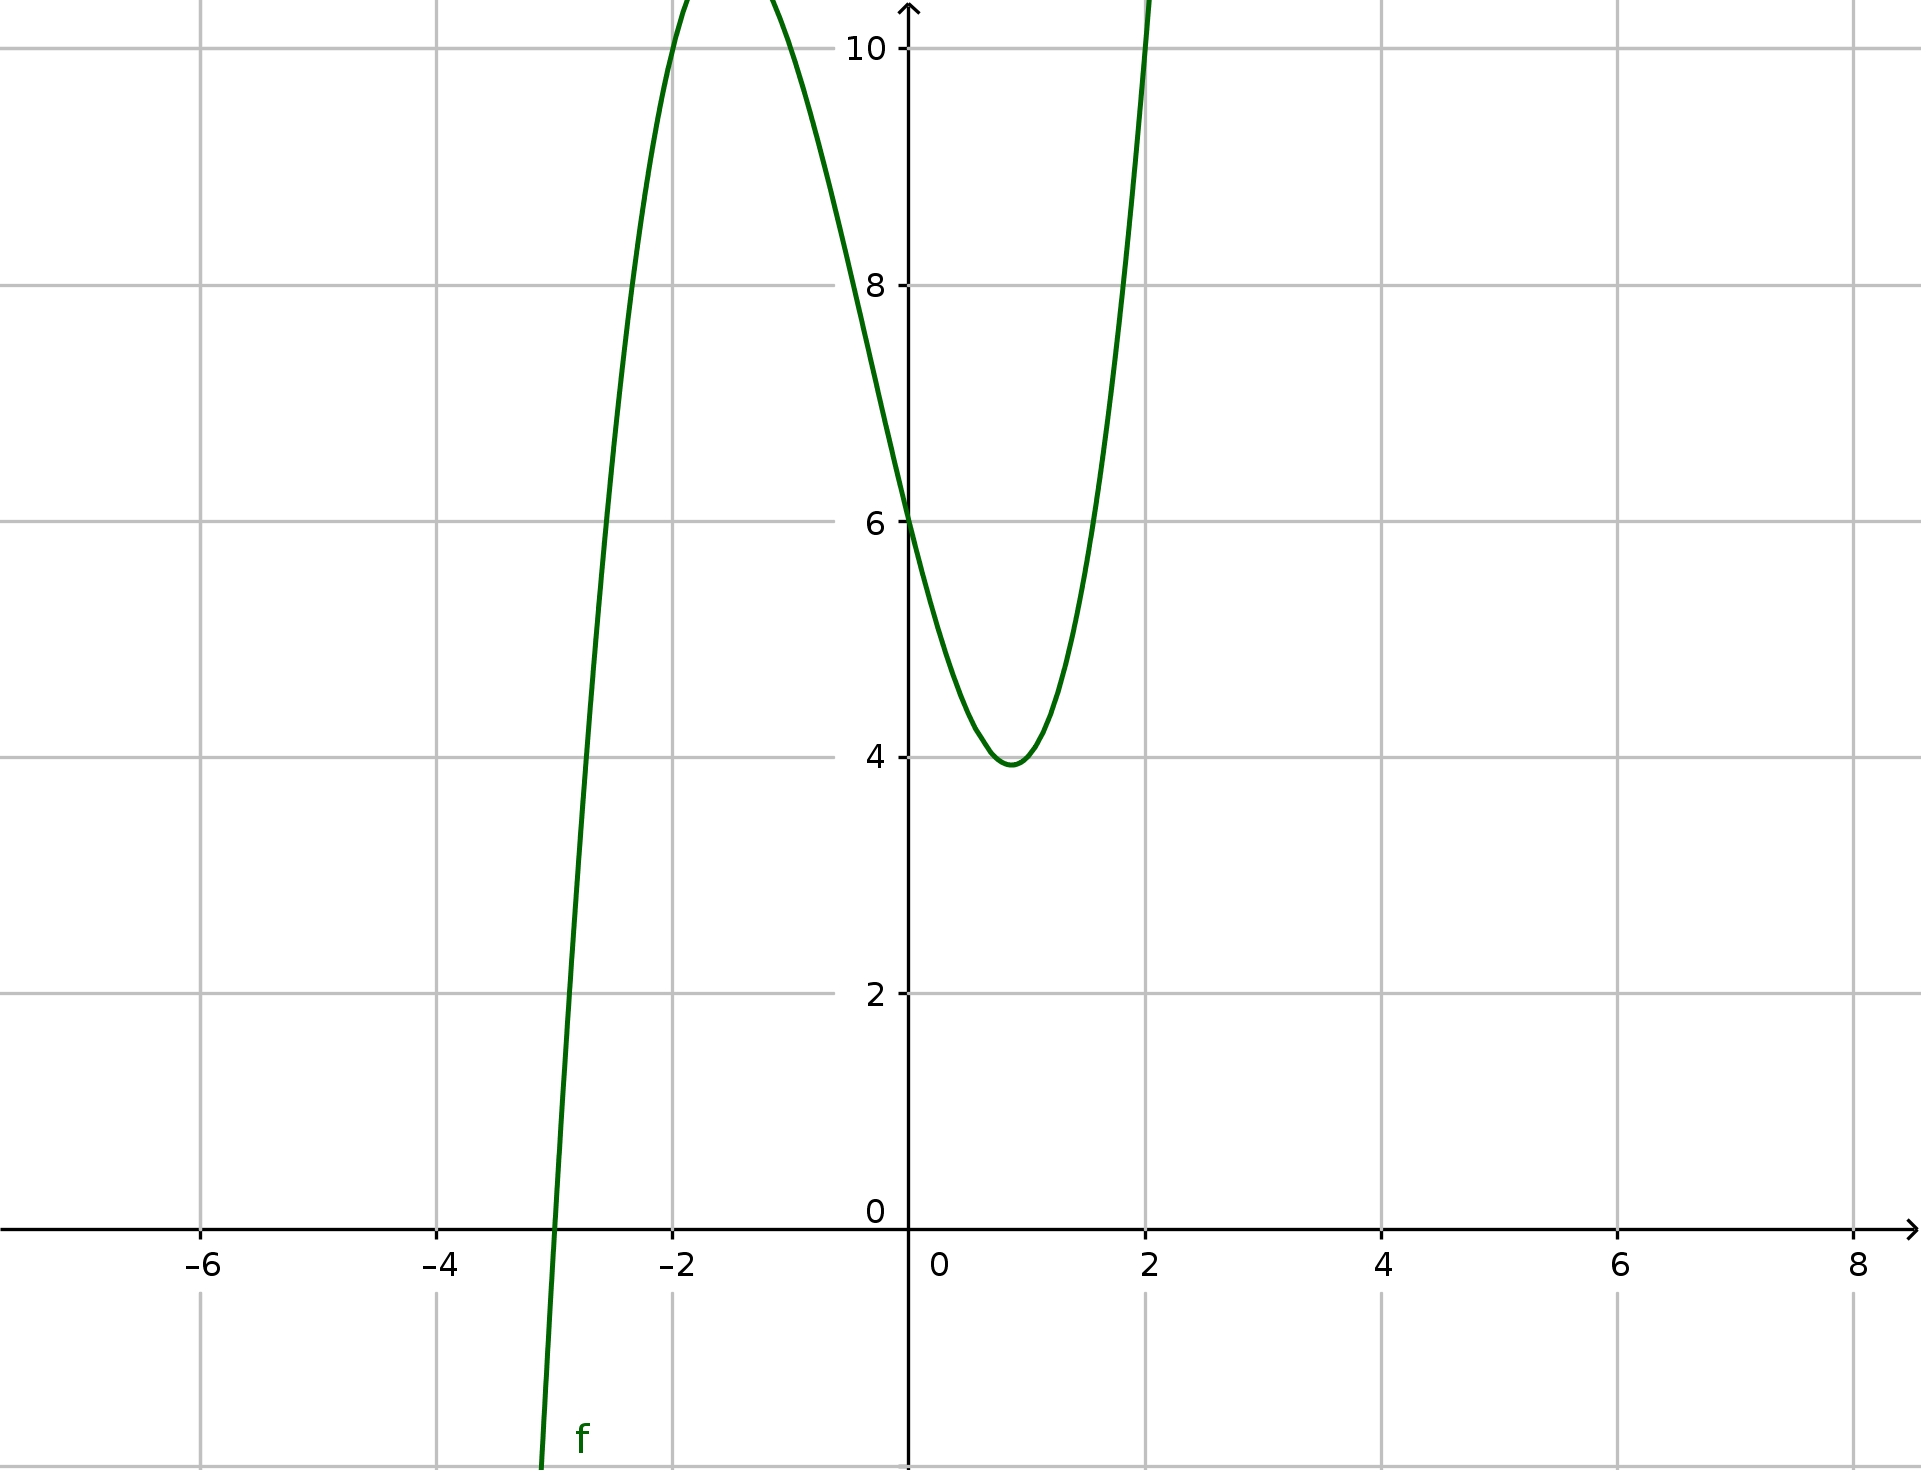
\includegraphics[width=120mm]{img1.png}
    \caption{Exercício 1}
    \end{figure}

    \begin{figure}[h!]
    \centering
    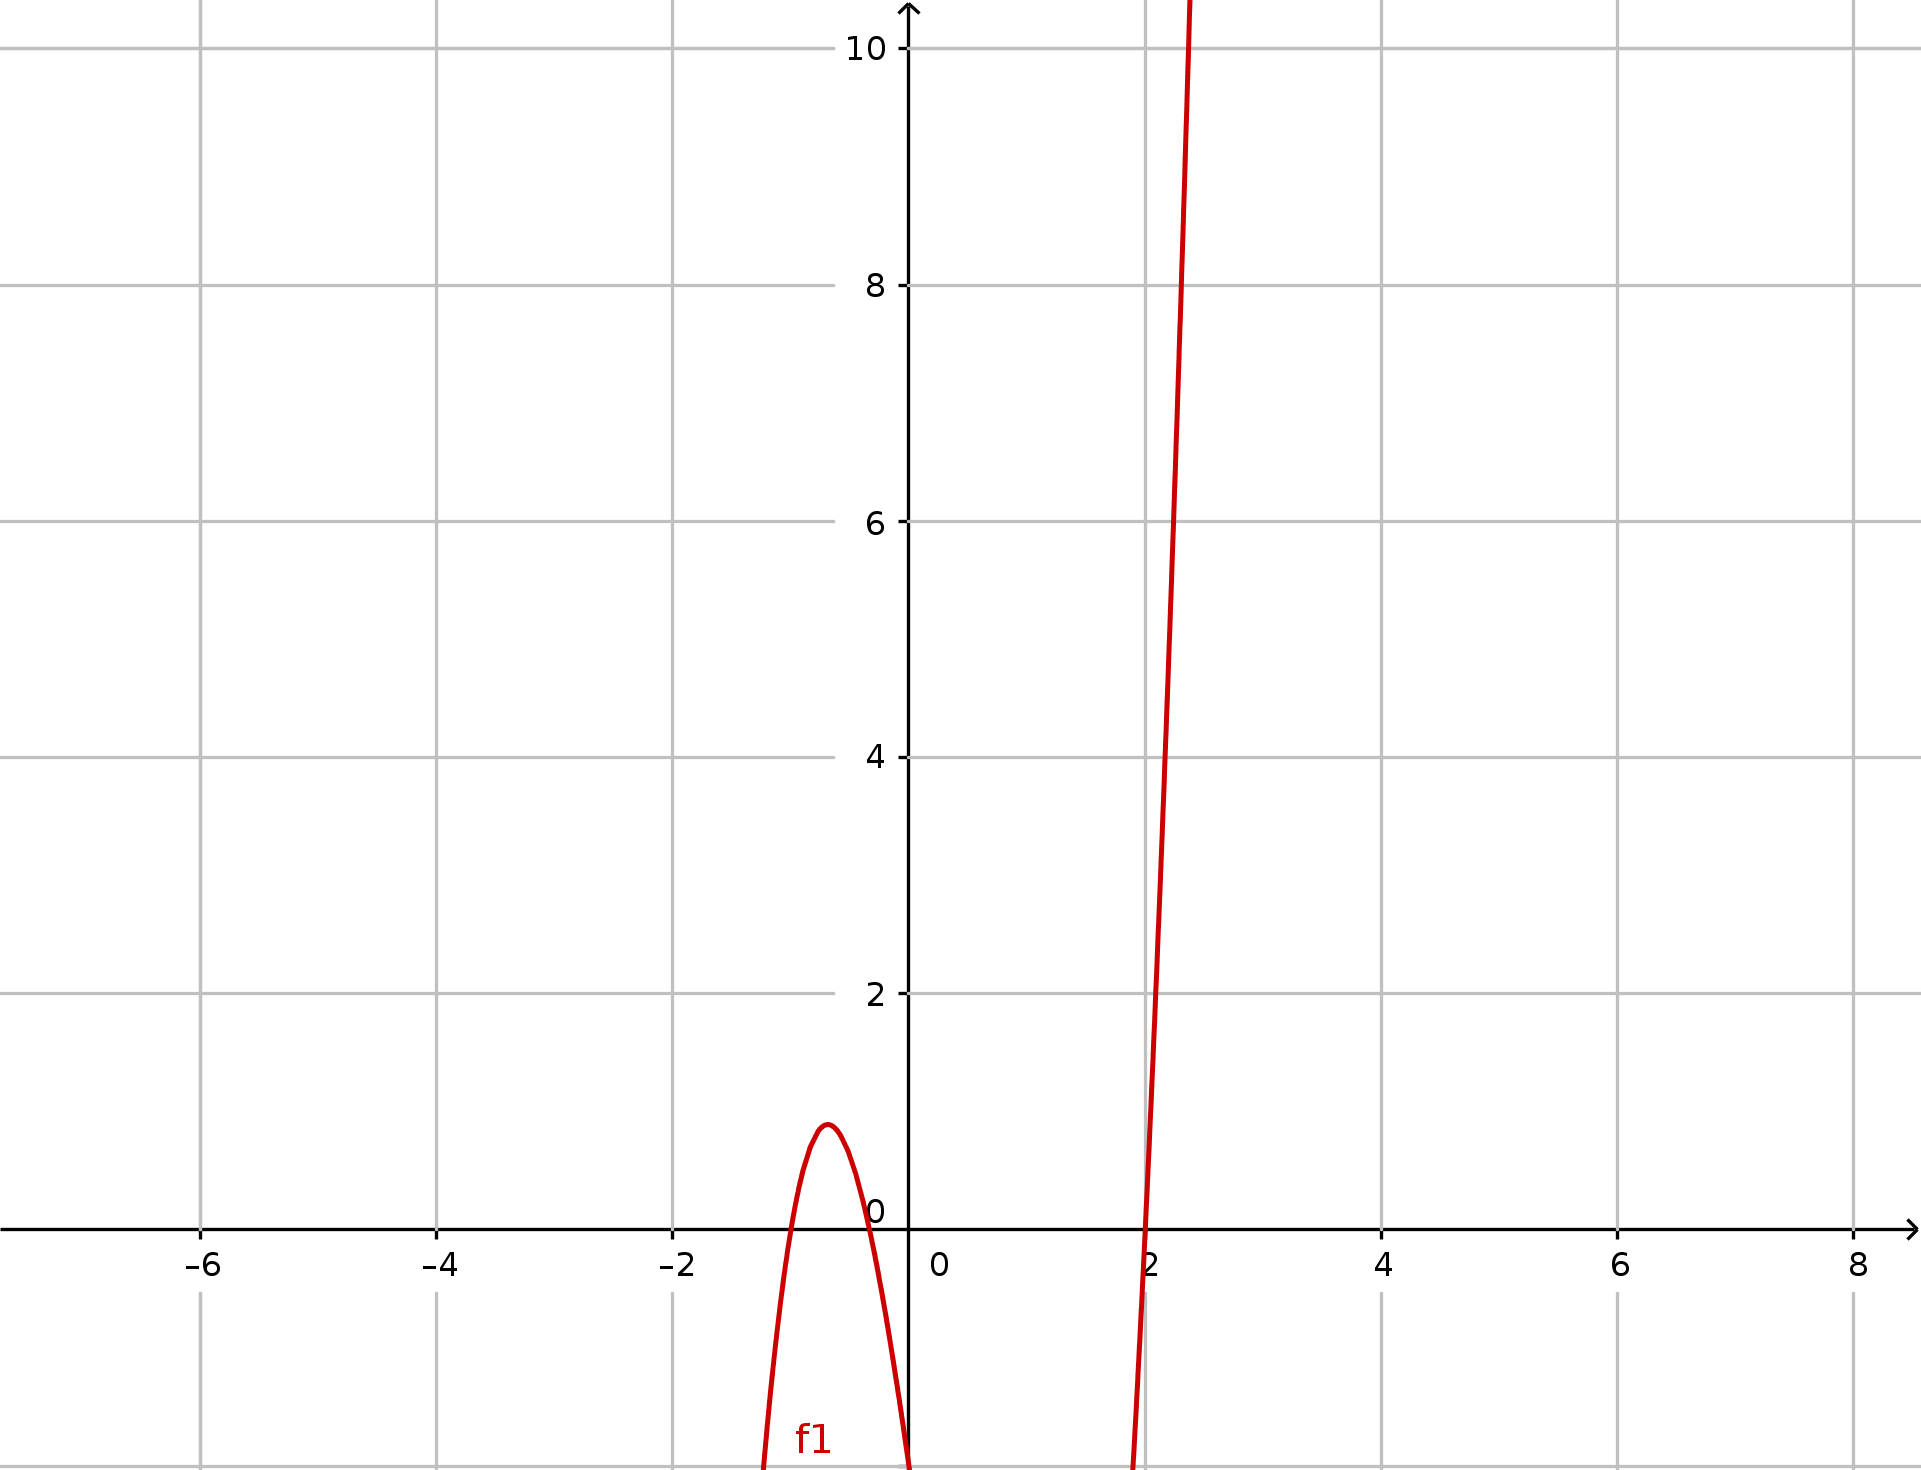
\includegraphics[width=120mm]{img2.png}
    \caption{Exercício 2}
    \end{figure}

    \begin{figure}[h!]
    \centering
    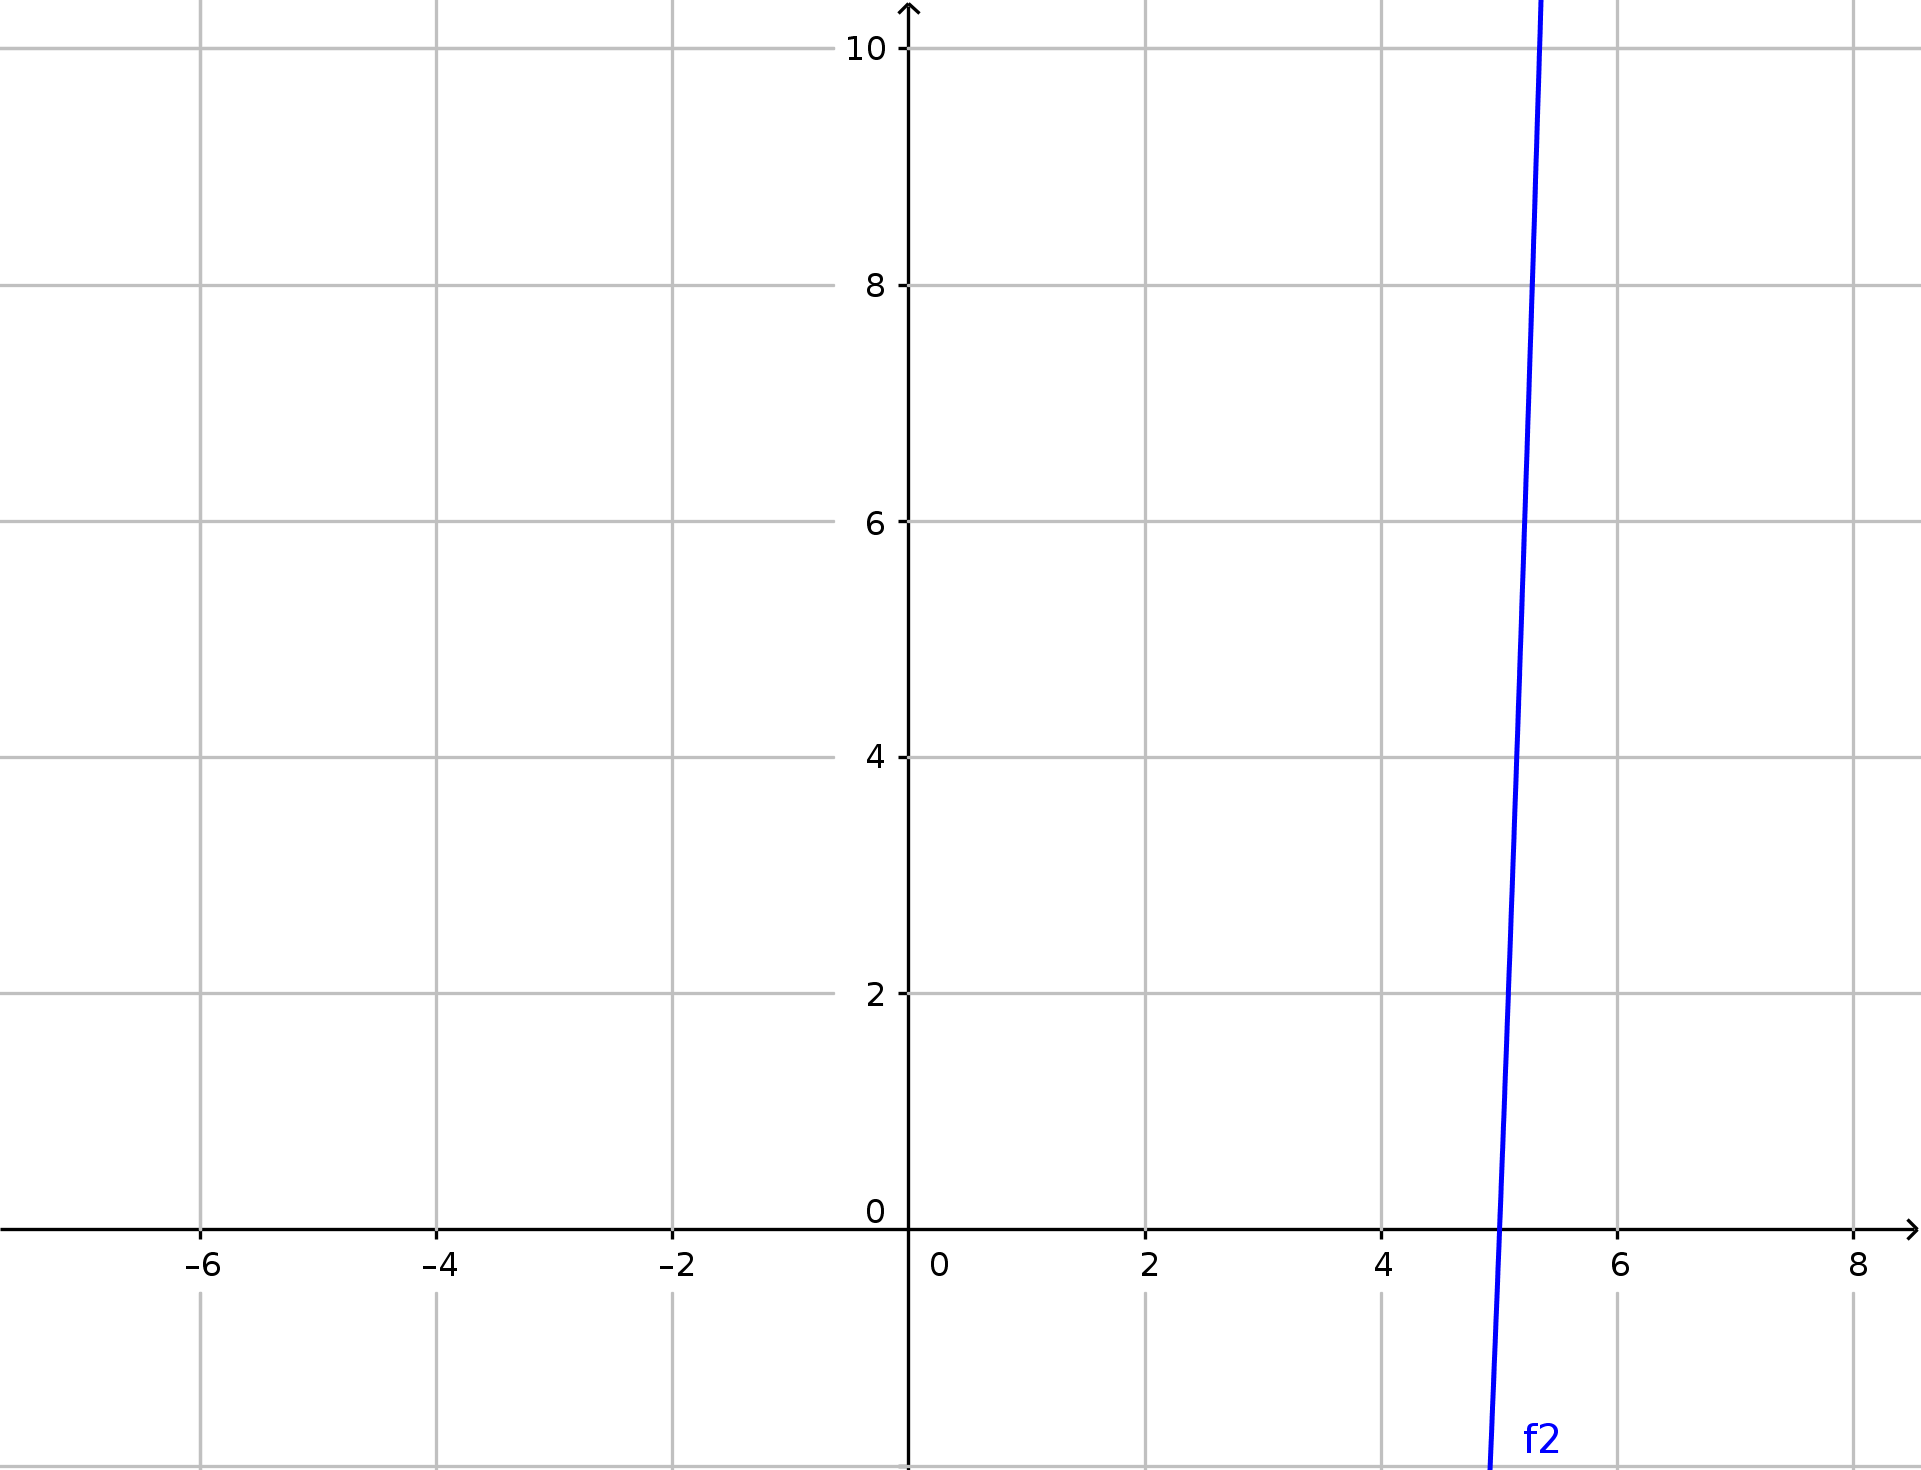
\includegraphics[width=120mm]{img3.png}
    \caption{Exercício 3}
    \end{figure}

    \begin{figure}[h!]
    \centering
    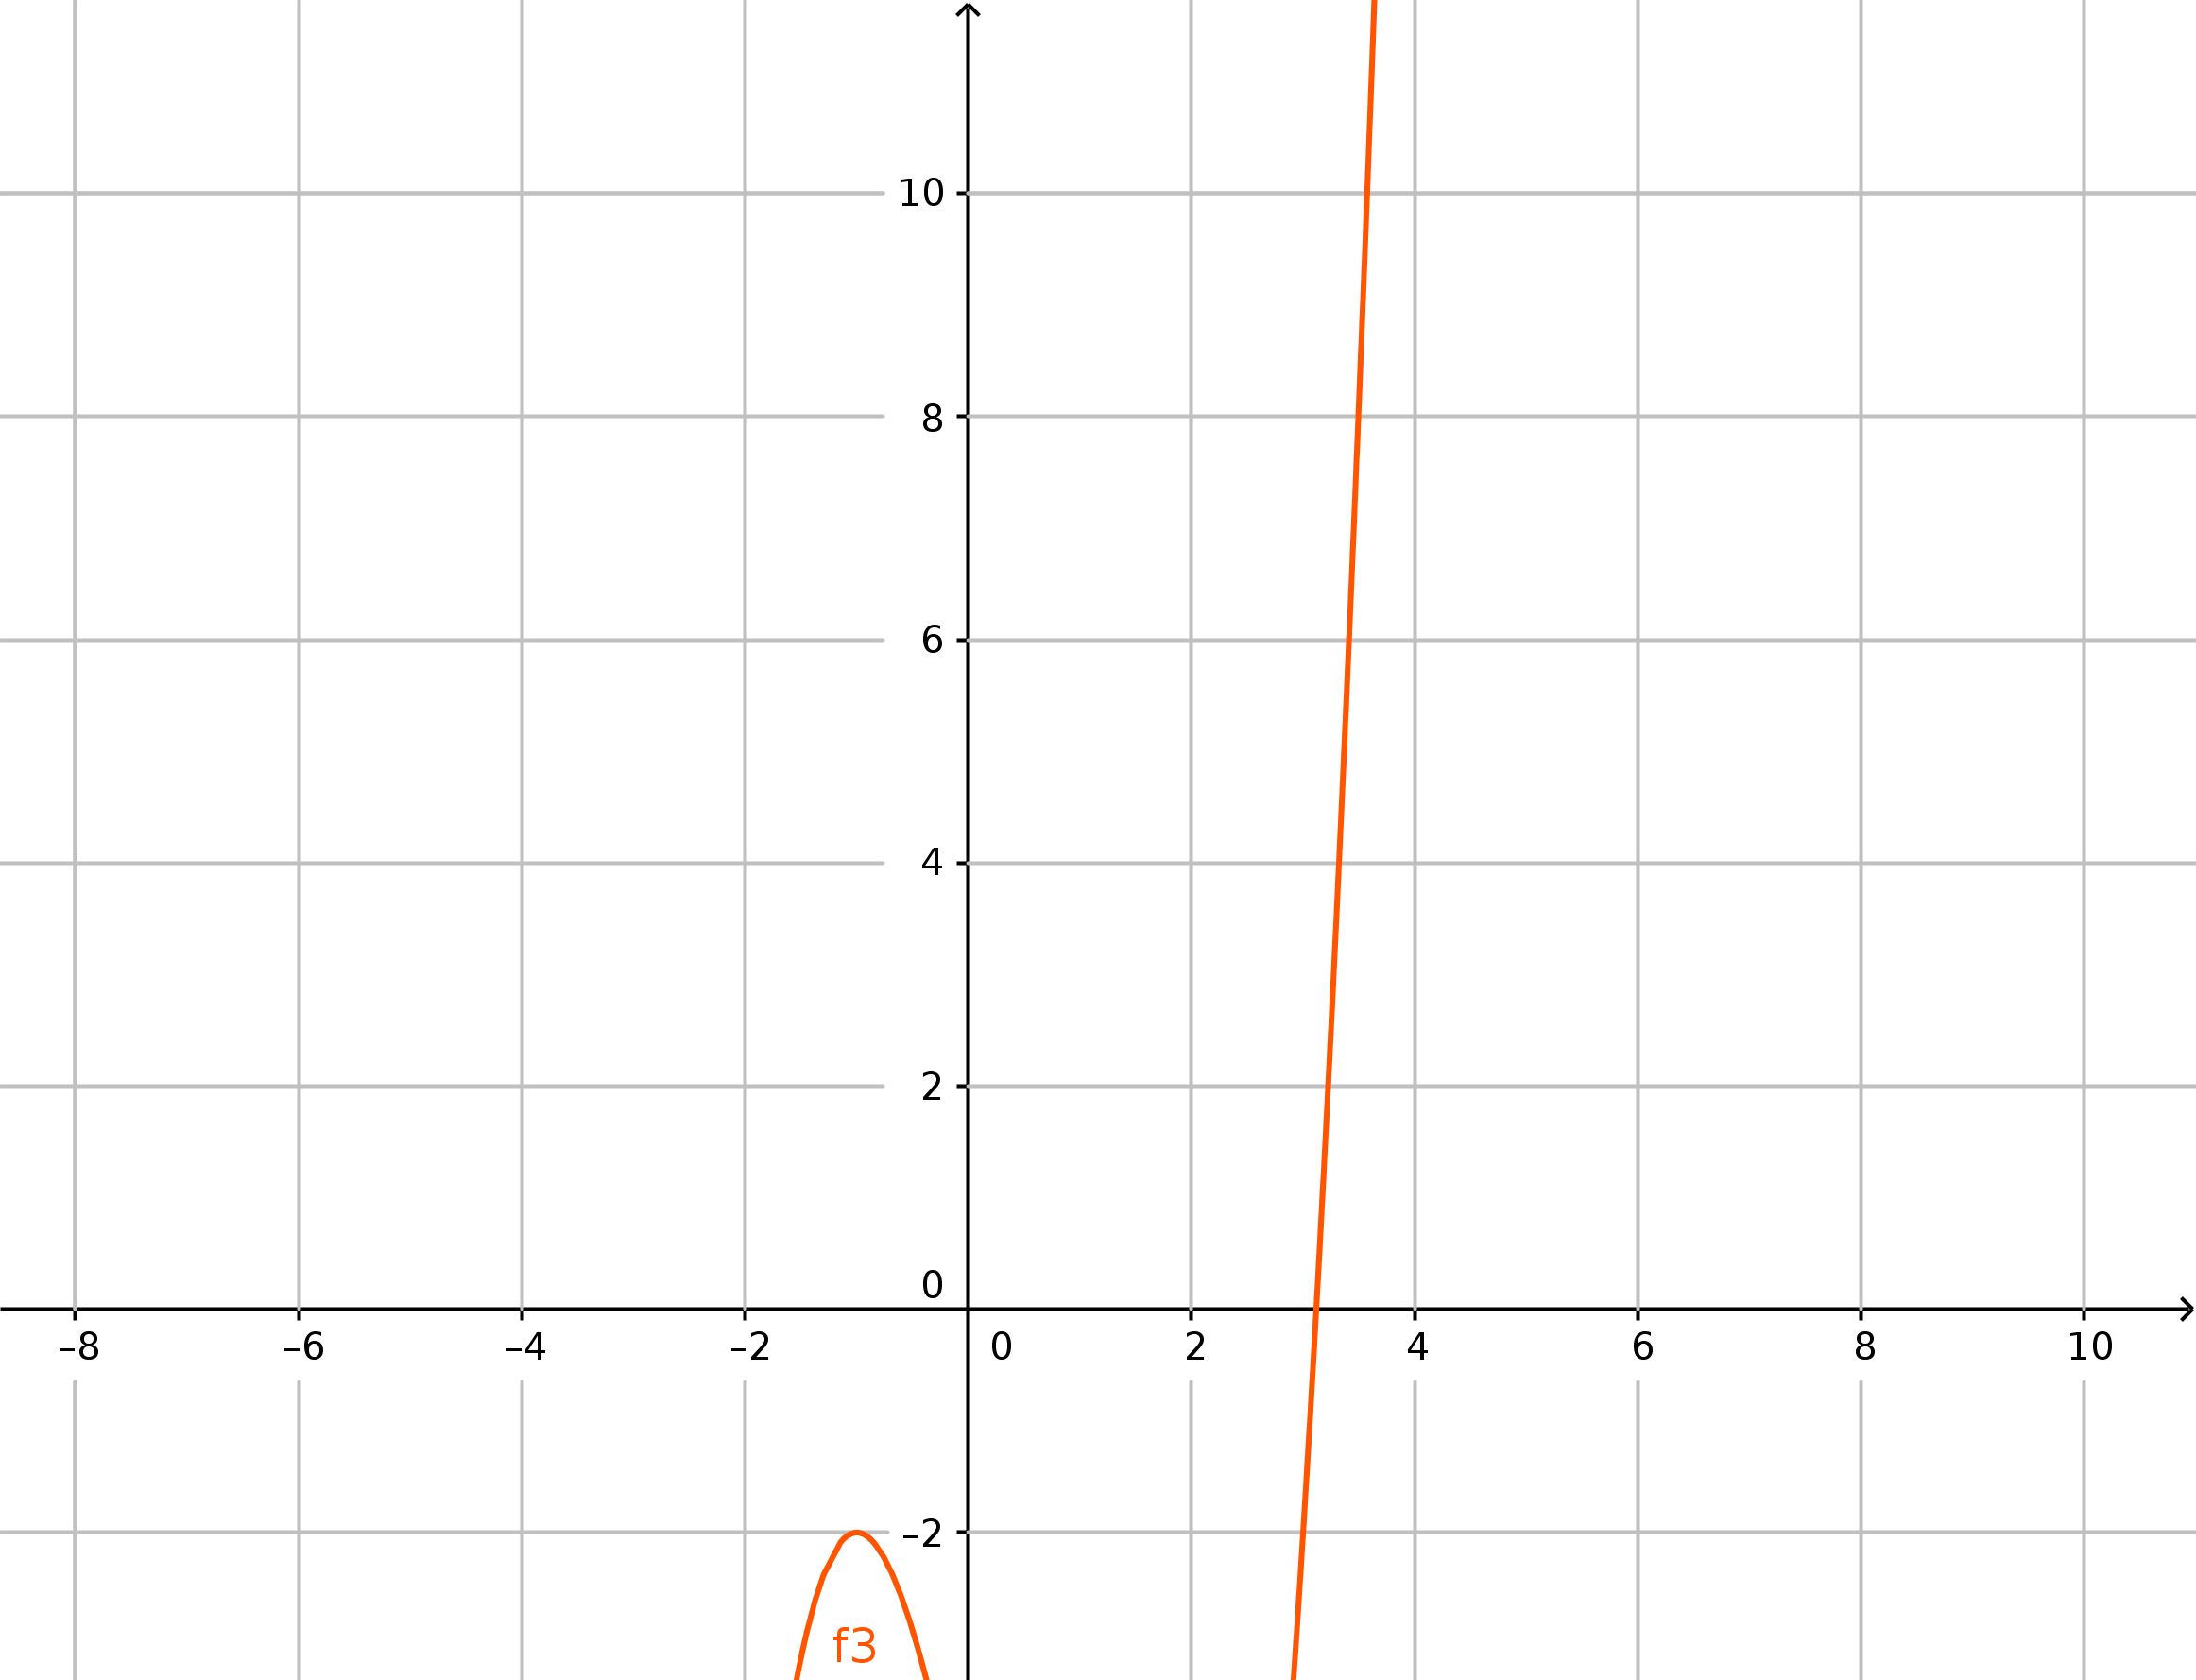
\includegraphics[width=120mm]{img4.png}
    \caption{Exercício 4}
    \end{figure}

    \begin{figure}[h!]
    \centering
    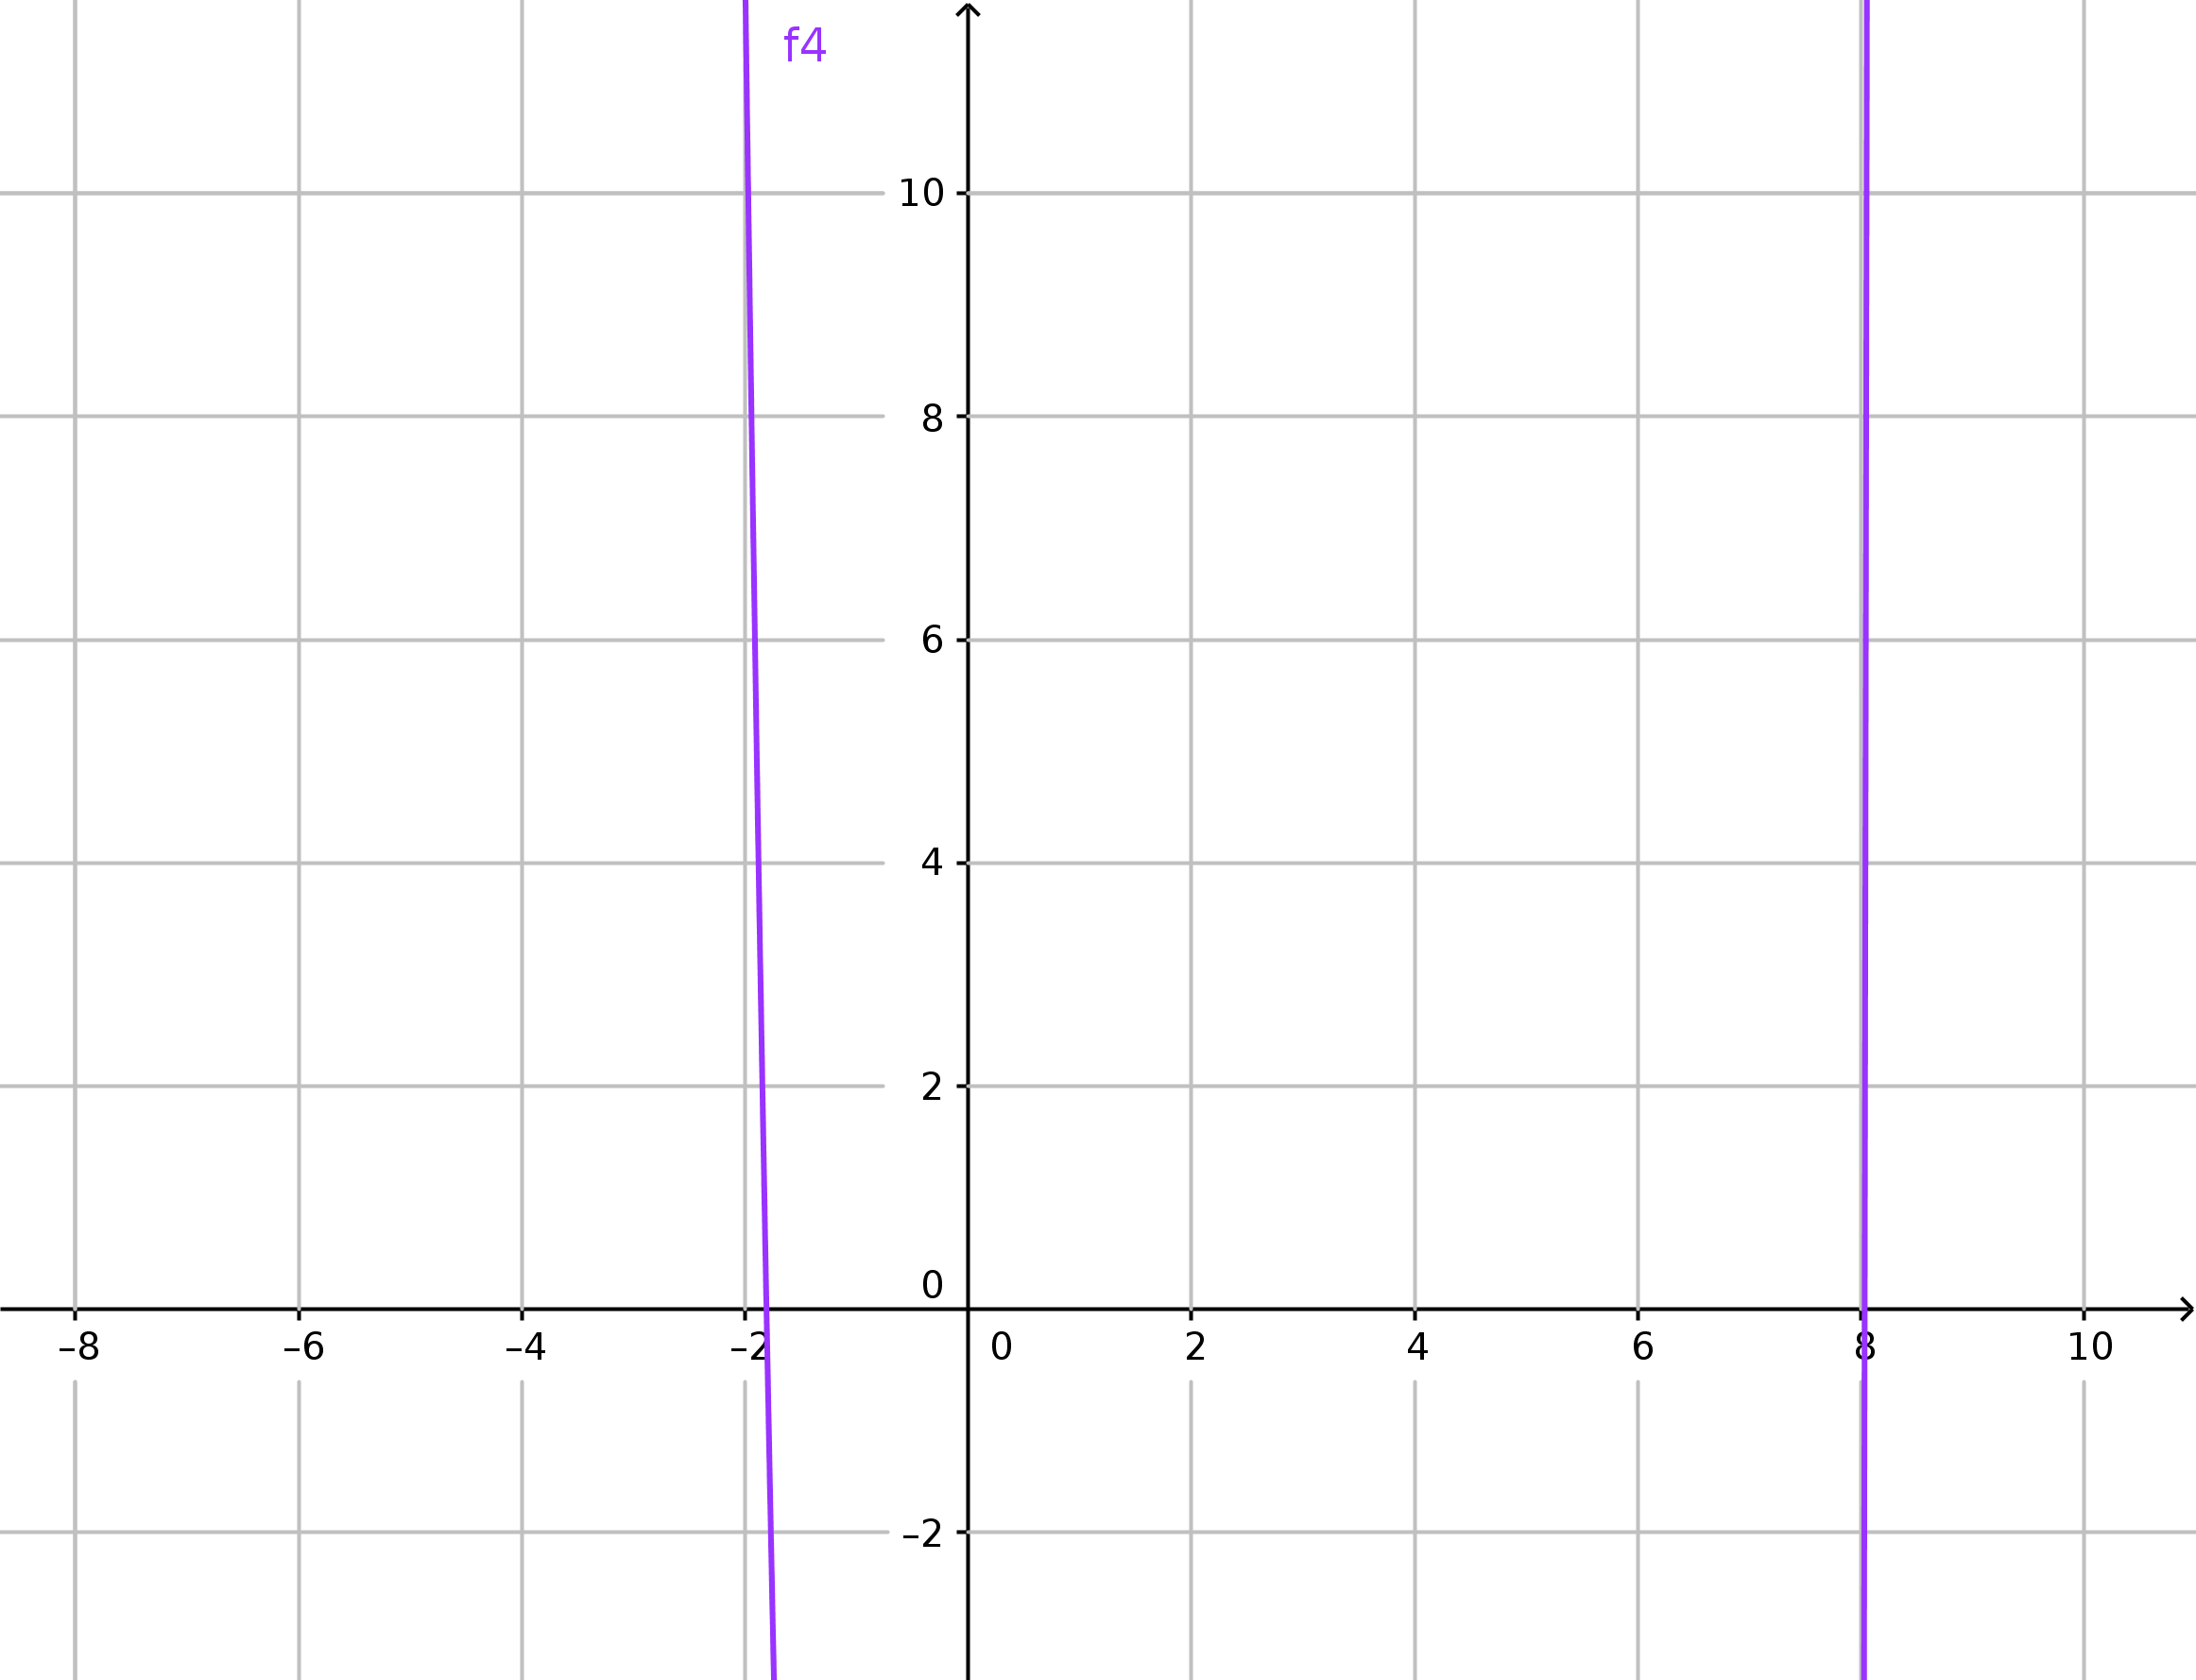
\includegraphics[width=120mm]{img5.png}
    \caption{Exercício 5}
    \end{figure}

\end{enumerate}
\end{document}
